
\documentclass[11pt, DINA4, fleqn]{amsart}

\pagestyle{empty}

\usepackage[english]{babel}
\usepackage[T1]{fontenc} 
\usepackage[utf8]{inputenc}
\usepackage{lmodern}
\usepackage{blindtext}
\usepackage{multirow}
\usepackage{booktabs}
\usepackage{faktor}
\usepackage{tikz}
\usepackage{fancybox,framed}
\usepackage{framed}
\usepackage{tcolorbox}

\usepackage{amsmath,amssymb,amsthm,amsfonts}
\usepackage{pifont}
\usepackage{dsfont}
\usepackage{enumitem}
\usepackage{wasysym}

\usepackage{geometry}
\geometry{hmargin=2.5cm,vmargin={2cm,1cm}}

\newcommand{\R}{\Bbb{R}}

\newtheorem{thm}{Frage}



\definecolor{mycolor}{rgb}{0.122, 0.435, 0.698}

\usepackage{xcolor}
\definecolor{darkgreen}{rgb}{0.14,0.72,0.31}
\definecolor{MyBoxColor}{rgb}{0.9,0.9,0.9}

\definecolor{NGreen}{rgb}{0.0,0.53,0.0}

\definecolor{CiteBlue}{RGB}{28, 58, 189}

\newenvironment{shadedSmaller}{
  \def\FrameCommand{\fboxsep=\FrameSep \colorbox{MyBoxColor}}
  \MakeFramed {\advance\hsize-2\width\FrameRestore}}
{\endMakeFramed}

\newtcolorbox{mybox_tc2}[1]{colback=red!5!white,colframe=red!75!black,fonttitle=\bfseries,title=#1}

\newtcolorbox{mybox_tc3}[1]{colback=darkgreen!5!white,colframe=darkgreen!75!black,fonttitle=\bfseries,title=#1}

\newenvironment{shadedSmallerPadding}{
  \def\FrameCommand{\fboxsep=0.15cm \colorbox{MyBoxColor}}
  \MakeFramed {\advance\hsize-1.1\width\FrameRestore}}
{\endMakeFramed}


\usetikzlibrary{matrix,arrows}


\newcommand{\Ldot}{\overset{\textbf{.}\kern0.23em}{\mathbf{L}}}



\def\df{\mathrm{d}\xspace}
\newcommand{\dd}[2]{\frac{\df#1}{\df#2}}
\newcommand{\ddd}[2]{\frac{\df^2#1}{\df#2^2}}
\newcommand{\dddd}[2]{\frac{\df^3#1}{\df#2^3}}
\newcommand{\ddddd}[2]{\frac{\df^4#1}{\df#2^4}}

\def\vr{\boldsymbol{r}\xspace}
\def\vrd{\dot{\vr}\xspace}
\def\vrdd{\ddot{\vr}\xspace}
\def\vrddd{\dddot{\vr}\xspace}
\def\vrp{{\vr}'\xspace}
\def\vrpp{{\vr}''\xspace}
\def\vbp{{\vb}'\xspace}
\def\vt{\boldsymbol{t}\xspace}
\def\vn{\boldsymbol{n}\xspace}
\def\vb{\boldsymbol{b}\xspace}
\def\vf{\boldsymbol{f}\xspace}

\usepackage{hyperref} % load hyperref as last package!

\hypersetup{
	colorlinks,
	linkcolor= CiteBlue,
	citecolor = CiteBlue,
	urlcolor=NGreen
}


\begin{document}

\begin{flushleft}
{\sc \LARGE A primer on differential geometry} \hfill \today \\
\medskip
\Large
Nikolas Schnellbächer \underline{\hspace{6.53in}} \\
\end{flushleft}

This set of notes contains a condensed review of some essential topics in differential geometry. 
It is meant as a short but concise review of some core concepts with an emphasis on a consistent presentation and full derivations of all statements and results
where possible.

\section{Differential geometry of curves}
\subsection{Arc length and tangent vector of a curve}

We consider a parametric curve $\vr = \vr(t)$, parametrized by a parameter $t$.
For most purposes we will consider three dimensional space curves
\begin{align}
\vr(t) = \bigl(x_1(t),\, x_2(t),\, x3(t)\bigl)^{\text{T}}\in \mathbb{R}^3 \, ,
\end{align}
however many of the introduced concepts are in fact more general.

Consider two points $P$ (at $\vr(t)$) and $Q$ (at $\vr(t+ \Delta t)$) on this curve, which are connected by the segment $\Delta\vr = \vr(t+\Delta t) - \vr(t)$, as illustrated in figure \ref{fig:figure_01}\hyperref[fig:figure_01]{A}. The length of this segment $\Delta s$, which connects both points, can then be approximated as
\begin{align}
\Delta s &\simeq |\Delta \vr| = 
\left| \vr(t + \Delta t) - \vr(t)
\right| \simeq
\left|
\vr(t) + \dd{\vr(t)}{t}\, \Delta t + \dfrac{1}{2}\ddd{\vr(t)}{t}\, (\Delta t)^2 + \dots
- \vr(t)
\right| \\
&= 
\left|
\dd{\vr(t)}{t}\, \Delta t + \dfrac{1}{2}\ddd{\vr(t)}{t}\, (\Delta t)^2
\right|
\simeq \left|\dd{\vr}{t}\right| \, \Delta t \, ,
\end{align}
where we use a Taylor expansion of $\vr(t+\Delta t)$ for small $\Delta t$. In short, we find the first order approximation
\begin{align}
\Delta s \simeq \left|\dd{\vr}{t}\right| \, \Delta t
\end{align}
from which we obtain the differential arc length $ds$ of the curve $\vr$ as
\begin{align}
ds = \left|\dd{\vr}{t}\right| \, dt
= \left|\vrd\right| \, dt = \sqrt{\vrd \cdot \vrd} \,\, dt \, .
\label{eq:diffArc}
\end{align}
At this point we emphasize
that we use dotted derivatives to denote derivatives of the curve $\vr$ with respect to its curve parameter $t$, \textit{i.e.} we define
\begin{align}
\vrd \equiv \dd{\vr(t)}{t} \, .
\end{align}

%%%%%%%%%%%%%%%%%%%%%%%%%%%%%%%%%%%%%%%%%%%%%%%%%%%%%%
\begin{figure}[h]
\centering
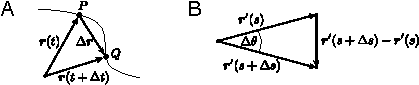
\includegraphics[width=0.70\textwidth]{./figures/figure_01}
\caption{\textbf{A} Two points along a curve $\vr$ which are connected by a segment $\Delta\vr$, whose length $\Delta s$ is used to define the arc length $s$ of a curve. \textbf{B} The tangential vector at a points $s$ and a second points $s+\Delta s$ from an isosceles triangle.}
\label{fig:figure_01}
\end{figure}
%%%%%%%%%%%%%%%%%%%%%%%%%%%%%%%%%%%%%%%%%%%%%%%%%%%%%%

It is very crucial to be notationally consistent.
In particular when we introduce abbreviations for derivatives, which is commonly done to avoid cluttered notation, at the risk of misuse and being more error prone.

Next, we consider a segment of the curve $\vr$ between the parameter $t_0$ and $t$, \textit{i.e.} between the two points $\vr(t_0)$ and $\vr(t)$.
We define the arc length of this segment as
\begin{align}
s(t) = \int\displaylimits_{t_0}^{t} \, ds = \int\displaylimits_{t_0}^{t} \,
\sqrt{\vrd \cdot \vrd} \,\, dt
= \int\displaylimits_{t_0}^{t}\sqrt{\dot{x}^2(t) + \dot{y}^2(t) + \dot{z}^2(t)} \,\, dt \, ,
\label{eq:arcLength}
\end{align}
which is valid provided there is a one-to-one mapping $\tau \in[t_0,t] \longmapsto \vr(\tau)$.
The vector $\dd{\vr}{t} = \vrd$ is called the tangent vector of the curve at this particular point. For all regular points of the curve $\vr$, this tangent vector is a vector with a finite magnitude. Revisiting the expression for the differential of the arc length in equation \eqref{eq:diffArc}, we can determine the magnitude of the tangent vector as
\begin{align}
\left|\vrd\right| \equiv \left|\dd{\vr}{t}\right| = \dd{s}{t} \, .
\end{align}
$|\vrd| = \dot{s}$ specifies the rate of change of the arc length $s$ as a function of the curve parameter $t$. For this reasons $|\vrd| = \dot{s} =:v$ is also called the parametric speed $v$.

\begin{mybox_tc3}{\emph{Parametric speed $v$} of a curve}
For a curve $\vr = \vr(t)$, the magnitude of its tangent vector 
quantifies the rate of change of the curve's arc length $s$ with respect to the curve parameter $t$ and is thus called parametric speed $v$.
\begin{align}
v := \dd{s}{t} = \left|\vrd\right| \equiv \left|\dd{\vr}{t}\right|
\label{eq:parametricSpeed}
\end{align}
When the parametric speed equal unity, \textit{i.e.} when
\begin{align}
\dd{s}{t} = 1 \, ,
\end{align}
the curve is said to be arc length parametrized. One equally refers to this curve as having unit speed.
This makes it clear, that instead of the arbitrary parameter $t$ one can equally use the arc length $s$ to parametrize a curve $\vr$.
\end{mybox_tc3}

The arc length $s$ of a curve $\vr$ as defined in equation \eqref{eq:arcLength} 
is independent of the parametrization that was chosen. We
show this property by restating equation \eqref{eq:arcLength} and introducing
a new arbitrary speed parametrization $u$, such that there is a one-to-one mapping
$t\mapsto u(t)$.
\begin{align}
s(t) = \int\displaylimits_{t_0}^{t} \, ds = \int\displaylimits_{t_0}^{t} \,
|\vrd| \,\, dt = 
\int\displaylimits_{t_0}^{t} \left|\dd{\vr}{t}\right| dt
= \int\displaylimits_{u_0 = u(t_0)}^{u=u(t)} \left|\dd{\vr}{u}\right|\left|\dd{u}{t}\right| dt
= \int\displaylimits_{u_0}^{u} \left|\dd{\vr}{u}\right| du
= s(u(t))
\label{eq:arcLengthIndependent}
\end{align}
Above I apologize for the ambiguity in notation by having $t$ (and likewise $u$) both as upper integration limit as well as independent integration variable and hope that it is clear how to distinguish them. I felt that introducing new properly labeled variables would over complicate things in this context and become in particular confusing, as we use primes do denotes derivatives with respect to the arc length $s$. 
Equation \eqref{eq:arcLengthIndependent} nicely illustrates that $s$ is independent of the parametrization and at the same times underlines the special role the arc length $s$ itself takes as a choice for a natural parametrization with unit speed.
By looking at how the arc length $s$ changes with the arbitrary curve parameter $t$, we find that
\begin{align}
\dot{s} = \dd{s(t)}{t} = \dd{}{t} \int\displaylimits_{t_0}^{t} |\vrd(t)|\,  dt = |\vrd| > 0 \quad \Longrightarrow \quad \dot{s}>0
\end{align}
holds for all non-singular points of a curve. This confirms that $s$ itself can indeed be used to parametrize the curve $\vr$ since it increases strictly with $t$, which allows us to invert $s = s(t)$ and obtain $t = t(s)$.
Sometimes a parametrization by arc length is also abbreviated as \emph{PARC} = Parametrization by ARC length.

By normalizing the tangent vector $\vrd$ we obtain the unit tangent vector $\vt$
\begin{align}
\vt = \dfrac{\vrd}{\left|\vrd\right|}
\equiv \dd{\vr}{t} \biggl/ \left|\dd{\vr}{t}\right|
= 
\dd{\vr}{t} \biggl / \dd{s}{t}
= \dd{\vr}{s} \equiv \vrp \, ,
\label{eq:tangent}
\end{align}
where we in the last step introduced the primed derivatives to denote derivatives with respect to the arc length $s$.
Reiterating the previous statement about notational consistency, make sure to distinguish between 
\begin{equation}
\vrd \equiv \dd{\vr}{t} \qquad \text{and} \qquad\vrp \equiv \dd{\vr}{s} \, .
\end{equation}
To get our head around having both the arc length $s$ and the independent non-arc length parameter $t$ at the same time, we next derive some basic relations between the two, by computing derivatives of them with respect to each other. We start by calculating the derivatives of the arc length $s$ with respect to $t$.
\begin{align}
\dot{s} &= \dd{s}{t} = \left|\vrd\right| = \sqrt{\vrd \cdot \vrd} \qquad \text{parametric speed (see
eqs. \eqref{eq:diffArc} and \eqref{eq:parametricSpeed})} \\
\ddot{s} &= \dd{\dot{s}}{t} = \dd{}{t}\left( \sqrt{\vrd \cdot \vrd}\right)
= \dfrac{1}{2 \sqrt{\vrd \cdot \vrd}} \left[\dd{}{t}\left(\vrd\cdot \vrd\right)\right]
= \dfrac{1}{2 \sqrt{\vrd \cdot \vrd}} \left[\vrd \cdot \vrdd +\vrdd \cdot \vrd \right] =
\dfrac{\vrd\cdot\vrdd}{\sqrt{\vrd \cdot \vrd}} \\
\dddot{s} &= \dd{\ddot{s}}{t} = \dfrac{\vrdd\cdot\vrdd + \vrd\cdot\vrddd}{\sqrt{\vrd \cdot \vrd}} - (\vrd\cdot\vrdd)\dfrac{1}{2} \dfrac{(\vrd \cdot \vrdd + \vrdd \cdot \vrd)}{(\vrd \cdot \vrd)^{3/2}}
= \dfrac{(\vrd\cdot\vrd)(\vrdd\cdot\vrdd + \vrd\cdot\vrddd) - (\vrd\cdot\vrdd)^2}{(\vrd\cdot\vrd)^{3/2}}
\end{align}
In a similar fashion we compute the first three derivatives of $t$ with respect to $s$.
\begin{align}
t' &\equiv \dd{t}{s} = \dfrac{1}{|\vrd|} = \dfrac{1}{\sqrt{\vrd \cdot \vrd}}  \qquad \text{(see
	eqs. \eqref{eq:diffArc} and \eqref{eq:parametricSpeed})} \\
t'' &= \dd{t'}{s} = \dd{}{s}\left(\left(\vrd\cdot\vrd\right)^{-1/2}\right) = -\dfrac{1}{2\left(\vrd\cdot\vrd\right)^{3/2}}\, 2\vrd\cdot \left(\dd{}{s}\vrd\right)
= \dfrac{-\vrd\cdot \left(\left(\dd{}{t}\vrd\right) \, \left(\dd{t}{s}\right)\right)}{\left(\vrd\cdot\vrd\right)^{3/2}}
= - \,\dfrac{\vrd\cdot \vrdd}{\left(\vrd\cdot\vrd\right)^{2}} \\
t''' &= \dd{t''}{s} = \left(\dd{t''}{t}\right) \,\left(\dd{t}{s}\right) = \dfrac{1}{\sqrt{\vrd\cdot\vrd}} \, \dd{}{t}\left(- \,\dfrac{\vrd\cdot \vrdd}{\left(\vrd\cdot\vrd\right)^{2}} \right) \\
&= \dfrac{-1}{\sqrt{\vrd\cdot\vrd}}\left[
\dfrac{\vrdd\cdot\vrdd + \vrd\cdot\vrddd}{(\vrd\cdot\vrd)^2} + (\vrd\cdot\vrdd) \dfrac{(-2)\cdot \, 2 \cdot \, (\vrd\cdot\vrdd)}{(\vrd\cdot\vrd)^3}
\right]
= \dfrac{-(\vrdd\cdot\vrdd + \vrd\cdot \vrddd)(\vrd\cdot\vrd) + 4(\vrd\cdot\vrdd)^2}{(\vrd\cdot\vrd)^{7/2}}
\end{align}

\subsection{Example: Semi-cubical parabola}
We have a look at the curve
\begin{align}
\vr(t) = \begin{pmatrix}
t^2 \\ t^3
\end{pmatrix}.
\end{align}
For the non-unit tangent vector we find
\begin{align}
\dd{\vr(t)}{t} = \begin{pmatrix}
2t \\ 3t^2
\end{pmatrix}
\end{align}
and thus its parametric speed is
\begin{align}
v = |\vrd| = \left|\dd{\vr}{t}\right| = \sqrt{4t^2 + 9t^4} = \sqrt{t^2(4+9t^2)} \, .
\end{align}
From this we can tell that $|\vrd| = 0$ only occurs for $t=0$, \textit{i.e.} the curve is only singular at the origin.

\section{Principal normal and curvature}
\subsection{Principal normal}
Having introduced the arc length in the previous section, we will now make use of a curve in arc length parametrization, \textit{i.e.}
we look at a curve $\vr = \vr(s)$ and will see that the arc length parametrization has several useful properties.
For this reason the arc length parametrization of a curve is sometimes also referred to as \emph{natural parametrization}.
Having a second look at equation \eqref{eq:tangent}, we already showed that the derivative of $\vr$ with respect to its arc length $s$, can be written as a normalized vector
\begin{align}
\vrp \equiv \dd{\vr}{s} = \dfrac{\vrd}{|\vrd|} \, ,
\end{align}
from which we hence also can state, that the vector $\vrp(s)$ itself must be a unit vector ($|\vrp| = 1$).
We rewrite this normalization condition as
\begin{align}
\vrp \cdot \vrp = |\vrp|^2 = 1
\end{align}
and subsequently take the derivative of this equation with respect to the arc length $s$ to find
\begin{align}
\vrpp \cdot \vrp + \vrp\cdot \vrpp = 2\vrp\cdot\vrpp = 0 \quad \Longrightarrow \quad \vrp \cdot \vrpp = 0 \, .
\end{align}
This orthogonality condition $\vrp\cdot \vrpp = 0$ tells us that $\vrpp$ is orthogonal/normal to the tangent vector $\vrp = \vt$.
With this observation we define the unit vector
\begin{align}
\vn = \dfrac{\vrpp(s)}{|\vrpp(s)|} \equiv \dfrac{\vt'(s)}{|\vt'(s)|}
\label{eq:normalVector}
\end{align}
as \emph{unit principal normal vector} at $s$. The plane spanned by the tangent vector $\vt(s)$ and the principal normal vector $\vn(s)$
is called \emph{osculating plane} at that point.

\subsection{Curvature $\kappa$}
Comparing the tangent vectors $\vrp(s)$ at $s$ with the tangent vector $\vrp(s+\Delta s)$ at $s + \Delta s$, we notice, that they together with
their difference vector $\vrp(s+\Delta s) - \vrp (s)$ from an isosceles triangle (see figure \ref{fig:figure_01}\hyperref[fig:figure_01]{B}). Since we are currently working in arc length parametrization, we have that both
tangent vectors have unit norm, \textit{i.e.} $|\vrp(s)| = 1 = |\vrp(s+ \Delta s)|$. Using $\Delta \theta$ to denote the angle between the two tangent vectors
$\vrp(s)$ and $\vrp(s+\Delta s)$, we find the relation
\begin{align}
|\vrp(s+\Delta s) - \vrp(s)| = |\vrp(s + \Delta s)| \, \Delta\theta = 1 \cdot \Delta \theta = |\vrpp(s) \, \Delta s| \, ,
\label{eq:curvatureDerivation1}
\end{align}
for small $\Delta s\longrightarrow 0$.
Here we used that
\begin{align}
\frac{\Delta \theta}{2} \simeq \sin\left(\frac{\Delta \theta}{2}\right) = \dfrac{|\vrp(s + \Delta s) - \vrp(s)|}{2\, |\vrp(s+ \Delta s)|} = \dfrac{|\vrp(s + \Delta s) - \vrp(s)|}{2}
\end{align}
holds for the isosceles triangle shown in figure \ref{fig:figure_01}\hyperref[fig:figure_01]{B},
combined with the fact that we can write the second derivative of $\vr$ with respect to $s$ as
\begin{align}
\vrpp(s)  = \lim_{\Delta s\rightarrow 0} \, \dfrac{\vrp(s+\Delta s) - \vrp(s)}{\Delta s} \, .
\end{align}
From equation \eqref{eq:curvatureDerivation1} we get
\begin{align}
|\vrpp(s)| = \lim_{\Delta s\rightarrow 0} \, \dfrac{\Delta \theta}{\Delta s} =
\lim_{\Delta s\rightarrow 0} \, \dfrac{\Delta \theta}{\rho \Delta \theta}  = \dfrac{1}{\rho} =: \kappa
\end{align}
We call $\kappa$ curvature and its inverse $1/\kappa = \rho$ the radius of curvature at $s$.
Combining this new expression for the curvature with our previous result for the principal normal unit vector $\vn$
as defined in equation \eqref{eq:normalVector}, we obtain
\begin{align}
\vrpp(s) \equiv \vt'(s) = |\vrpp(s)|\,  \vn(s) = \kappa(s) \, \vn(s) \, ,
\end{align}
identifying the curvature $\kappa$ as the magnitude of $\vrpp(s)$.

\begin{mybox_tc3}{\emph{Curvature} and \emph{curvature vector}}
	For a curve in arc length parametrization $\vr = \vr(s)$, the vector
	\begin{align}
	\vrpp(s) \equiv \vt' \equiv \ddd{\vr}{s}
	\end{align}
	is called \emph{curvature vector} and measures the rate of change of the tangent along the curve.
	Its magnitude $|\vrpp(s)| =: \kappa$ is called curvature and its inverse is better known as the radius of curvature $\rho = 1/\kappa$.
	By definition $\kappa$ is non-negative.
	The radius of curvature $\rho(s) = 1/\kappa(s)$ is sometimes also called the radius of the so-called ``kissing circle'' at that specific point.
	The normalized curvature vector
	\begin{align}
	\vn = \dfrac{\vrpp(s)}{|\vrpp(s)|} \equiv \dfrac{\vt'(s)}{|\vt'(s)|}
	\equiv \dfrac{1}{\kappa}\dd{\vt(s)}{s}
	\label{eq:normalVectorBox}
	\end{align}
	is called \emph{unit principal normal vector} and is a normalized vector which is always normal to the tangent vector $\vt(s)$ in $s$, \textit{i.e.}
	$\vn\cdot\vt = 0 \Longleftrightarrow \vn \perp \vt$.
\end{mybox_tc3}

\subsection{Curvature for an arbitrary speed curve}
In the previous section on the principal normal vector and curvature we assumed our curve $\vr$ to be parametrized by its
arc length, allowing us to obtain expression for the unit principal normal vector and the curvature $\kappa$.
Here we show how to obtain an expression for the curvature for an arbitrary speed curve, \textit{i.e.} a curve which is parametrized by an arbitrary parameter $t$, which is not the arc length (for non-arc length parametrized curves).

For this purpose we start by evaluating expressions for $\vrd$ and $\vrdd$ in terms of the arc length $s$ by applying the chain rule accordingly.
\begin{align}
\vrd = \dd{\vr}{t} = \dd{\vr}{s} \dd{s}{t} = |\vrd| \vt = v \vt \, ,
\end{align}
using the previous established relation for the parametric speed $v = |\vrd|$ from equation \eqref{eq:parametricSpeed}.
\begin{align}
\vrdd = \dd{}{t}\left(v\vt\right) = \vt \dd{v}{t} + v\dd{\vt}{t} = \vt \dd{v}{t} + v \dd{\vt}{s}\dd{s}{t}
= \vt \dd{v}{t} + v^2 \underbrace{\dd{\vt}{s}}_{=\kappa \vn} = \left(\dd{v}{t}\right) \, \vt + v^2\kappa \, \vn
\end{align}
By taking the cross product of $\vrd$ with $\vrdd$ we obtain
\begin{align}
\vrd \times \vrdd = v\vt \times \left[
\left(\dd{v}{t}\right) \, \vt + v^2\kappa \, \vn
\right]
= v^3\kappa \biggl(\vt \times \vn \biggl) \, .
\label{eq:curvatureDerivation2}
\end{align}
Taking the absolute value, we get
\begin{align}
\left|\vrd\times\vrdd\right| = |\vrd|^3 \kappa \underbrace{|\vt \times\vn|}_{= 1} = |\vrd|^3 \kappa \, ,
\label{eq:curvatureDerivation3}
\end{align}
which we can then isolate for the curvature $\kappa$.
\begin{mybox_tc3}{\emph{Curvature} for an arbitrary speed curve}
	The curvature of an arbitrary speed curve $\vr = \vr(t)$ is
	given by
	\begin{align}
	\kappa = \dfrac{|\vrd\times\vrdd|}{|\vrd|^3} = \dfrac{|\vrd\times\vrdd|}{v^3} \, ,
	\end{align}
	where $v = |\vrd|$ is the parametric speed of the curve.
\end{mybox_tc3}
In the derivation of this result we used the fact, that $\vt \times \vt = 0$ and that the cross product of two unit vectors results again in a unit vector ($|\vt\times\vn| = 1$).

\section{Binormal vector and torsion}
We already stated the result, that the tangent vector $\vt(s)$ and the principal unit normal $\vn(s)$ are perpendicular unit vectors ($\vt\cdot\vn = 0$), which together span the \emph{osculating} plane in a point $s$. We complement this set of two vectors by a third unit binormal vector $\vb$, such that the set
$(\vt, \vn, \vb)$ forms a right-handed screw, \textit{i.e.} they satisfy the cyclic relation
\begin{align}
\vb = \vt \times \vn \qquad \vt = \vn \times \vb \qquad \vn = \vb \times \vt \, .
\label{eq:tnbScrew}
\end{align}
Below we state the names of the planes which are spanned by all combinations of two out of theses three, respectively.
\begin{align}
(\vt, \vn) \quad &\text{span the osculating plane} \\
(\vn, \vb) \quad &\text{span the normal plane} \\
(\vb, \vt) \quad &\text{span the rectifying plane}
\end{align}
For a curve in arc length parametrization, equation \eqref{eq:normalVectorBox} states how to obtain the unit principal normal vector $\vn$ and using the first equation from \eqref{eq:tnbScrew} we also get the binormal unit vector $\vb$. For arbitrary speed curves it is on the contrary a priori not clear how to compute $\vn$ and $\vb$.
It turns out, that it is relatively easy to find an expression for the binormal unit vector $\vb$.
We recall equation \eqref{eq:curvatureDerivation2}, where we had
\begin{align}
\vrd \times \vrdd
= v^3\kappa \biggl(\underbrace{\vt \times \vn}_{=\vb} \biggl)
\end{align}
which we rearrange to get
\begin{align}
\vb = \dfrac{\vrd \times \vrdd}{v^3 \kappa} = \dfrac{\vrd \times \vrdd}{|\vrd \times \vrdd|} \, ,
\end{align}
also making use of $v^3\kappa = |\vrd\times\vrdd|$ according to equation \eqref{eq:curvatureDerivation3}.
In summary, for arbitrary speed curves with non-zero curvature, one can find the binormal unit vector as
\begin{align}
\vb = \dfrac{\vrd \times \vrdd}{|\vrd \times \vrdd|}.
\end{align}
From there we also get the principal normal unit vector $\vn$ for arbitrary speed curves
by $\vn = \vb \times \vt$.

\begin{mybox_tc3}{{Tangent, normal and binormal unit vectors for normal and arbitrary speed parametrizations}}
	Summarizing some of the result from the last sections, we state below how to calculate the unit tangent, the unit principal normal and the unit binormal vector for both arc-length and arbitrary speed parametrized curves $\vr$.
	\begin{align}
	&\vt(s) = \dd{\vr(s)}{s} = \vrp(s)
	&\vt(t) = \dd{\vr(t)}{t} \biggl/ \left|\dd{\vr(t)}{t}\right| = \dfrac{\vrd}{|\vrd|} \\
	&\vn(s) = \dfrac{\vrpp(s)}{\kappa} = \dfrac{\vrpp(s)}{|\vrpp(s)|} \equiv \dfrac{\vt'(s)}{|\vt'(s)|}
	& \vn(t) = \vb(t) \times \vt(t) \\
	&\vb(s) = \vt(s)\times \vn(s)
	&\vb(t) =  \dfrac{\vrd \times \vrdd}{|\vrd \times \vrdd|}
	\end{align}
\end{mybox_tc3}

The binormal vector $\vb$ is perpendicular to the osculating plane by construction $\vb = \vt \times \vn$.
Now we investigate its rate of change.
\begin{align}
\vbp \equiv \dd{\vb}{s} = \dd{}{s}\left(\vt \times \vn\right) = \underbrace{\dd{\vt}{s}}_{=\vt' = \kappa \vn} \times \vn + \vt \times \dd{\vn}{s}
= \kappa \underbrace{\vn\times\vn}_{=\boldsymbol{0}} + \, \vt \times \dd{\vn}{s} = \vt \times \vn'
\end{align}
Thus we get $\vb' = \vt \times \vn'$.

The principal normal vector $\vn$ is a unit vector $|\vn| = 1$, \textit{i.e.} $\vn \cdot \vn = 1$.
As before we can derive an orthogonality relation from this normalization condition, by taking the derivative of both sides with respect to $s$.
\begin{align}
\dd{}{s}(\vn\cdot\vn)  = 2\, \vn\cdot\vn'= \dd{}{s}(1) = 0 \quad \Longrightarrow \quad \vn \cdot \vn' = 0
\end{align}
From this we learn that $\vn'$ is parallel to the rectifying plane spanned by $(\vb, \vt)$.
That is to say, that there exist some coefficients $\mu$ and $\tau$, such that we can write
\begin{align}
\vn' =\mu\vt + \tau \vb \, .
\label{eq:nprimeExp}
\end{align}
Having found this representation for $\vn'$ we go back to the rate of change of the binormal vector and find
\begin{align}
\vb' = t\times \vn' = \vt \times \left(\mu \vt + \tau \vb\right) = \tau \left(\vt \times \vb\right) = - \tau \underbrace{\left(\vb\times \vt\right)}_{=\vn}
= -\tau\vn
\label{eq:bprimeExp}
\end{align}
The coefficient $\tau$ is called torsion and measures how much the curve $\vr$ deviates from the osculating plane spanned by $(\vt, \vn)$.
\textit{I.e.} it measures how strongly the curve is twisted out of this plane.
Next, we take the dot product of $\vb' = -\tau\vn$ with $(-\vn)$ to get
\begin{align}
-\vn \cdot \vb' = + \tau\, \vn \cdot \vn =\tau
\end{align}
which we can isolate for the torsion $\tau$ giving 
\begin{align}
\tau = -\vn \cdot \vb' = -\vn \cdot \dd{\vb}{s} \, .
\end{align}
The relation above tells us how to calculate the torsion for a curve $\vr$ given in arc length parametrization.
This result can also be expressed in terms of derivatives of the curve vector $\vr$ itself.
\begin{align}
\tau = - \vn \cdot \vb' = -\dfrac{\vr''}{\kappa} \cdot \left[\dd{}{s}\left(\vt \times \vn\right)\right]
\end{align}
where we used $\vn = \vr'' /\kappa$  and $\vb = \vt \times \vn$. We continue by inserting $\vt = \vr'$ and obtain
\begin{align}
\tau &= -\dfrac{\vr''}{\kappa} \cdot \left[\dd{}{s}\left(\vr' \times \dfrac{\vr''}{\kappa}\right)\right] \\
&= -\dfrac{\vr''}{\kappa} \cdot \left[
\underbrace{\vr'' \times \dfrac{\vr''}{\kappa}}_{=\boldsymbol{0}} + \vr' \times \dd{}{s}\left(\dfrac{\vr''}{\kappa}\right)
\right] \\
&= -\dfrac{\vr''}{\kappa} \cdot \left[
\vr' \times \left(
\dfrac{1}{\kappa}\vr''' + \vr'' \dd{\kappa^{-1}}{s}
\right)
\right] \\
&= -\dfrac{\vr''}{\kappa} \cdot\left(
\vr' \times \dfrac{1}{\kappa} \vr'''
\right) \, ,
\end{align}
where we used the fact $\vr'' \cdot(\vr' \times \vr'') = 0$.
Using the cyclic permutations of the triple scalar product in the last expressions, we can write
\begin{align}
\tau = -\dfrac{1}{\kappa^2} \left(\vr''\times \vr'\right) \cdot \vr'''=
\dfrac{ \left(\vr'\times \vr''\right) \cdot \vr'''}{\kappa^2} = 
\dfrac{ \left(\vr'\times \vr''\right) \cdot \vr'''}{\vr''\cdot \vr''} \, ,
\label{eq:torsion1}
\end{align}
where we used $\kappa = |\vr''| = \sqrt{\vr''\cdot\vr''}$ and accordingly $\vr''\cdot \vr'' = \kappa^2$ in the last step.
This result for the torsion $\tau$, as shown in equation \eqref{eq:torsion1},  is once again only valid for arc length parametrized curves $\vr(s)$. Next, we use this result to derive the general expression for arbitrary speed curves, similar to like we did before for the curvature.
To do so, we restate some of our previous result, that we make use of to rearrange equation \eqref{eq:torsion1}.
For the denominator of equation \eqref{eq:torsion1} we use
\begin{align}
&\vr''\cdot\vr'' = \kappa^2 = \dfrac{|\vrd\times\vrdd|^2}{|\vrd|^6}
\end{align}
while we replace the derivatives of $\vr(s)$ in the numerator by their arbitrary speed counter parts.
\begin{align}
\vrp(s) &= \dd{\vr}{s} = \dfrac{\vrd}{|\vrd|} \qquad \text{(see equation \eqref{eq:tangent})} 
\label{eq:rpExp}\\
\vrpp(s) &= \dd{}{s}\left(\dd{\vr}{s}\right) = \dd{}{s}\left(\dd{\vr}{t} \, \cdot \, \dd{t}{s}\right)
= \left(\underbrace{\ddd{\vr}{t}}_{=\vrdd} \cdot \dd{t}{s}\right) \dd{t}{s} + \dd{\vr}{t} \cdot \ddd{t}{s}
\\
&= \vrdd \underbrace{\left(\dd{t}{s}\right)^2}_{=1/|\vrd|^2} + \vrd \left(\ddd{t}{s}\right)
= \dfrac{\vrdd}{|\vrd|^2} + \left(\ddd{t}{s}\right) \vrd
\label{eq:rppExp} \\
\vr'''(s) &= \dd{}{s}\left(
\ddd{\vr}{t} \cdot \left(\dd{t}{s}\right)^2
+ \dd{\vr}{t} \cdot \ddd{t}{s}
\right) \\
&= \dddd{\vr}{t} \left(\dd{t}{s}\right)^3 + \ddd{\vr}{t} \cdot 2 \left(\dd{t}{s}\right) \cdot \left(\ddd{t}{s}\right)
+ \ddd{\vr}{t}\left(\dd{t}{s}\right)\left(\ddd{t}{s}\right)
+ \dd{\vr}{t} \dddd{t}{s} \\
&= \dfrac{\vrddd}{|\vrd|^3} + 3 \left(\ddd{t}{s}\right)
\dfrac{\vrdd}{|\vrd|} + \left(\dddd{t}{s}\right) \vrd
\label{eq:rpppExp}\
\end{align}
Now we insert our results for $\vr'$, $\vr''$ and $\vr'''$ (equations \eqref{eq:rpExp}, \eqref{eq:rppExp} and \eqref{eq:rpppExp}) into the numerator of equation \eqref{eq:torsion1} and exploit several orthogonality relations, which ensure that from equation \eqref{eq:rppExp} only the term $\sim \vrdd$ remains and likewise from the expression in equation \eqref{eq:rpppExp} only the summand $\sim\vrddd$ stays. This leaves us with
\begin{align}
\tau =
\dfrac{ \left(\vr'\times \vr''\right) \cdot \vr'''}{\vr''\cdot \vr''} =
\dfrac{\left(\dfrac{\vrd}{|\vrd|} \times \dfrac{\vrdd}{|\vrd|^2}\right) \cdot \dfrac{\vrddd}{|\vrd|^3}  \, \cdot \,|\vrd|^6}{|\vrd \times \vrdd|^2}
= 
\dfrac{\left(\vrd \times \vrdd \right) \cdot \vrddd }{|\vrd \times \vrdd|^2}
= 
\dfrac{\left(\vrd \times \vrdd \right) \cdot \vrddd }{(\vrd \times \vrdd)\cdot (\vrd \times \vrdd)}.
\end{align}

\begin{mybox_tc3}{\emph{Torsion} of arc length and arbitrary speed curves}
The torsion $\tau$ for an arc length parametrized curve $\vr(s)$ is given as
\begin{align}
\tau(s) = \dfrac{ \left(\vr'\times \vr''\right) \cdot \vr'''}{\vr''\cdot \vr''} = \dfrac{ \left(\vr'\times \vr''\right) \cdot \vr'''}{|\vr''|^2}
\end{align}
where primed derivatives are taken with respect to the arc length $s$, $\vrp = \dd{\vr}{s}$. For arbitrary speed curves $\vr(t)$ the torsion is given as
\begin{align}
\tau(t) = 
\dfrac{\left(\vrd \times \vrdd \right) \cdot \vrddd }{(\vrd \times \vrdd)\cdot (\vrd \times \vrdd)}
=
\dfrac{\left(\vrd \times \vrdd \right) \cdot \vrddd }{|\vrd \times \vrdd|^2}
\end{align}
where dotted derivatives are taken with respect to the arbitrary speed parameter $t$, $\vrd= \dd{\vr}{t}$.
\end{mybox_tc3}
When working in arc length parametrization, the short hand expression for the torsion we derived was
\begin{align}
\tau= -\vn\cdot \dd{\vb}{s} = -\vn \cdot \vb' \, .
\end{align}
Revisiting equation \eqref{eq:nprimeExp} and taking the dot product with the unit vector $\vb$ we find
\begin{align}
\vn' &= \mu \vt + \tau \vb \\
\vn' \cdot \vb &= \mu\, \underbrace{\vt \cdot \vb}_{=0} + \tau\, \underbrace{\vb \cdot \vb}_{=1} \qquad \Longrightarrow \qquad \tau = \vb \cdot \dd{\vn}{s} \, .
\end{align}
That is, we obtain two very similar expressions for the torsion in arc length parametrization
\begin{align}
\tau = -\vn \cdot \vb' = + \vb \cdot \vn' \, .
\end{align}

\section{The comoving frame (Frenet frame)}
As established before, $\vt$, $\vn$ and $\vb$ form a set of three mutually perpendicular unit vectors. 
We also previously established that
$\vn(s) = \vt'(s) / \kappa$, which we can rearrange to get the first Frenet formula
\begin{align}
\dd{\vt(s)}{s} =  \kappa \, \vn(s) \, .
\end{align}
In our previous derivation for the torsion in equation \eqref{eq:bprimeExp} we also already derived an expression for $\vb'(s)$ which read
\begin{align}
\dd{\vb(s)}{s} = -\tau \, \vn(s) \, .
\end{align}
Next we revisit
\begin{align}
\vn' = \dd{}{s} \left(\vb \times \vt\right) &= \vb' \times \vt \, + \, \vb \times \vt' \\
&= -\tau \vn \times \vt \, + \, \vb \times \left(\kappa \vn\right) \\
&= \tau \, \underbrace{\vt \times \vn}_{=\vb} \, -  \, \kappa \, \underbrace{\vn\times\vb}_{=\vt}
= -\kappa \vt \, + \, \tau \vb \, .
\end{align}
We already wrote down an expression for $\vn'$ earlier in equation \eqref{eq:nprimeExp} as
\begin{align}
\vn' = \mu \vt + \tau \vb \, ,
\end{align}
allowing us to identify that the yet unidentified coefficient $\mu$ in fact turns out to be the curvature $\mu = \kappa$.
Summarizing the three relations for $\vt'$, $\vn'$ and $\vb'$ prime from the section thus far, we realize that we can write them down as a linear system.
This set of equations is well known as the \emph{Frenet-Serret} formulae.
\begin{mybox_tc3}{\emph{Frenet-Serret} formulae}
	The derivatives of the unit tangent, the unit principal normal and the unit binormal vector satisfy the following linear system, which in matrix form reads
\begin{align}
\begin{pmatrix}
\vt' \\ \vn' \\ \vb'
\end{pmatrix} = 
\begin{pmatrix}
0 & \kappa & 0\\
-\kappa & 0 & \tau \\
0 & - \tau & 0 
\end{pmatrix} 
\cdot
\begin{pmatrix}
\vt \\ \vn \\ \vb
\end{pmatrix} 
\end{align}
For an arbitrary speed parametrization, we realize that
\begin{align}
\vt' = \dd{\vt}{s} = \left(\dd{\vt}{t}\right) \left(\dd{t}{s}\right) = \dfrac{1}{v} \, \dot{\vt}
\end{align}
meaning that we can rewrite $\vt' = \kappa \vn$ as
$\dot{\vt} = v\kappa \vn$. Using that we can also write $\vn' = \dot{\vn}/v$ and $\vb' = \dot{\vb}/v$ we find the Frenet-Serret formulae for an arbitrary speed parametrization as
\begin{align}
\begin{pmatrix}
\dot{\vt} \\ \dot{\vn} \\ \dot{\vb}
\end{pmatrix} = 
\begin{pmatrix}
0 & v\kappa & 0\\
-v\kappa & 0 & v\tau \\
0 & - v\tau & 0 
\end{pmatrix} 
\cdot
\begin{pmatrix}
\vt \\ \vn \\ \vb
\end{pmatrix}  \, ,
\end{align}
where $v$ is the parametric speed of the curve as introduced before.
These equations show the special role of the curvature $\kappa$ and the torsion $\tau$ for space curves. For this reason the equations
\begin{align}
\kappa &= \kappa(s) \\
\tau &= \tau(s)
\end{align}
are called \emph{intrinsic equations} of the curve.
\end{mybox_tc3}


\section{Example: Helical curve}
We illustrate some of our concepts by calculating some of these quantities for a helical curve
\begin{align}
\vr(t) = \begin{pmatrix}
R\cos(\omega t) \\
R\sin(\omega t) \\
bt
\end{pmatrix} \in \mathbb{R}^3
\end{align}
with radius $R$ and pitch $z_0 = b \, 2\pi / \omega$, parametrized by a non-arc length parameter $t$. For the limiting case of $b\rightarrow 0$, the helix becomes a circle in the $x$-$y$ plane, and in the opposite case of $b\rightarrow \infty$ the helix turns into a straight line.
We start by calculating the tangent vector and the parametric speed of the helical curve.
\begin{align}
\vrd = \dd{\vr}{t} = \begin{pmatrix}
-R\omega \sin(\omega t) \\
R\omega \cos(\omega t) \\
b
\end{pmatrix}
\end{align}
The magnitude of $\vrd$ gives us the parametric speed
\begin{align}
v = |\vrd| = \sqrt{R^2\omega^2 + b^2} > R\omega
\label{eq:helixSpeed}
\end{align}
which is also constant (\textit{i.e.} not depending on the independent parametrization variable $t$)
From equation \eqref{eq:helixSpeed} we obtain
\begin{align}
\dd{s}{t} = v = \text{const.}\qquad \Longrightarrow \qquad s(t) = v t
\end{align}
which we of course can immediately invert to get $t(s) = s/v$. With this we can switch to the arc length parametrization of the helical curve
\begin{align}
\vr(s) = \begin{pmatrix}
R\cos(\omega s/v) \\
R\sin(\omega s/v) \\
bs/v
\end{pmatrix}
\end{align}
From here we calculate the unit tangent vector $\vt$ and check that it has indeed unit speed.
\begin{align}
\vt(s) = \dd{\vr(s)}{s} = 
\begin{pmatrix}
-\dfrac{R\omega}{v}\sin(\omega s/v) \\
\dfrac{R\omega}{v}\cos(\omega s/v) \\
b/v
\end{pmatrix} \quad \Longrightarrow \quad
|\vt| = \sqrt{\dfrac{R^2\omega^2}{v^2} + \dfrac{b^2}{v^2}}
= \dfrac{\sqrt{R^2\omega^2 + b^2}}{v} = \dfrac{v}{v} = 1
\end{align} 
\begin{align}
\dd{\vt(s)}{s} =\begin{pmatrix}
-\dfrac{R\omega^2}{v^2}\cos(\omega s/v) \\
-\dfrac{R\omega^2}{v^2}\sin(\omega s/v) \\
0
\end{pmatrix}
\end{align}
From this we can directly compute the curvature of the helix.
\begin{align}
\kappa(s) = \left|\dd{\vt(s)}{s}\right| = \sqrt{\dfrac{R^2\omega^4}{v^4}} = \dfrac{R\omega^2}{v^2} = \dfrac{R\omega^2}{R^2\omega^2 + b^2} = \dfrac{1}{R + \dfrac{b^2}{R\omega^2}} < \dfrac{1}{R}
\end{align}
We revisit the two limiting cases for $b$,
\begin{align}
\lim_{b\rightarrow 0} \kappa(s) &= \dfrac{1}{R} \qquad \text{(curvature of a circle)} \\
\lim_{b\rightarrow \infty} \kappa(s) &= 0
\end{align}
recovering the curvature of a planar circle and vanishing curvature in the limit for a straight line, as expected for both cases.
Next, we compute the torsion $\tau$ for the helix for which we first need to establish an expression for the principal unit normal $\vn(s)$ and the binormal $\vb(s)$.
\begin{align}
\vn(s) = \dfrac{1}{\kappa} \dd{\vt(s)}{s} = \dfrac{v^2}{R\omega^2}
\begin{pmatrix}
-\dfrac{R\omega^2}{v^2}\cos(\omega s/v) \\
-\dfrac{R\omega^2}{v^2}\sin(\omega s/v) \\
0
\end{pmatrix} =
\begin{pmatrix}
-\cos(\omega s/v) \\
-\sin(\omega s/v) \\
0
\end{pmatrix} \quad \Longrightarrow \quad |\vn(s)| = 1
\end{align}
\begin{align}
\vb = \vt \times \vn = 
\begin{pmatrix}
-\dfrac{R\omega}{v}\sin(\omega s/v) \\
\dfrac{R\omega}{v}\cos(\omega s/v) \\
b/v
\end{pmatrix}
\times
\begin{pmatrix}
-\cos(\omega s/v) \\
-\sin(\omega s/v) \\
0
\end{pmatrix}
=\begin{pmatrix}
\dfrac{b}{v}\sin(\omega s/v) \\
-\dfrac{b}{v}\cos(\omega s/v) \\
R\omega/v
\end{pmatrix}
\end{align}
Both $\vn$ and $\vb$ are unit vectors as required. Now we can eventually compute the torsion $\tau$
\begin{align}
\tau = -\vn(s) \cdot \dd{\vb(s)}{s}
= - \begin{pmatrix}
-\cos(\omega s/v) \\
-\sin(\omega s/v) \\
0
\end{pmatrix}\cdot
\begin{pmatrix}
\dfrac{b\omega}{v^2} \cos(\omega s/v) \\
\dfrac{b\omega}{v^2} \sin(\omega s/v) \\
0
\end{pmatrix}
= \dfrac{b\omega}{v^2} = \dfrac{b\omega}{R^2\omega^2 + b^2}
\end{align}
\begin{align}
\lim_{b\rightarrow 0} \tau(s) &=
\lim_{b\rightarrow 0} \left(\dfrac{\omega}{\dfrac{R\omega^2}{b} + b}\right) = 0 \\
\lim_{b\rightarrow \infty} \tau(s) &= 0
\end{align}
In both limiting cases for $b$ the torsion vanishes which is to be expected for a planar circle and a straight line.

\subsection{Recovering the parametric curve from the intrinsic curve equations}
Using the intrinsic equations $\kappa = \kappa(s)$ and $\tau = \tau(s)$ in conjunction with the Frenet-Serret formulae we can recover the parametric curve, that we started with. For this purpose, we restate the curvature and torsion for the helical curve
\begin{align}
\kappa = \dfrac{R\omega^2}{v^2} \qquad \text{and} \qquad \tau = \dfrac{b\omega}{v^2} \, ,
\end{align}
which are here both constant.
By differentiating the first Frenet-Serret formulae twice with respect to $s$ we find
\begin{align}
\dd{\vt}{s} &= \kappa \vn \\
\ddd{\vt}{s} &= \kappa \dd{\vn}{s} \\
\dddd{\vt}{s} &= \kappa \ddd{\vn}{s} \, .
\end{align}
Taking the derivative of the second Frenet-Serret formulae with respect to $s$ we obtain
\begin{align}
\ddd{\vn}{s} = -\kappa \dd{\vt}{s} + \tau\dd{\vb}{s} = -\kappa \dd{\vt}{s} - \tau^2 \vn \, ,
\end{align}
where we inserted the third Frenet-Serret formula in the last step.
Combining the third derivative of the tangent with our result for the second derivative of the principal normal $\vn$ we get
\begin{align}
\dddd{\vt}{s} &= \kappa \ddd{\vn}{s} = \kappa \left(
-\kappa \dd{\vt}{s} - \tau^2 \vn
\right) = -\kappa^2 \dd{\vt}{s} - \tau^2 \kappa \vn
= -\kappa^2 \dd{\vt}{s} - \tau^2 \dd{\vt}{s} = -(\kappa^2 + \tau^2) \dd{\vt}{s} \, ,
\end{align}
where we again used the first Frenet-Serret formula $\vn = \vt'/\kappa$.
Recalling that $\vt' = \dd{\vr}{s}$ we obtain the following fourth order differential equation for the curve $\vr$
\begin{align}
\ddddd{\vr}{s} + \left(\kappa^2 + \tau^2\right) \ddd{\vr}{s} = 0 \, .
\end{align}
First we simplify the constant coefficient
\begin{align}
\kappa ^2 + \tau^2 = \left(\dfrac{\omega}{v}\right)^2
\end{align}
such that we need to solve
\begin{align}
\ddddd{\vr}{s} +  \left(\dfrac{\omega}{v}\right)^2\ddd{\vr}{s} = 0 \, .
\end{align}
This vectorial differential equation has the general solution
\begin{align}
\vr(s) = \boldsymbol{C}_0 + \boldsymbol{C}_1 s
+ \boldsymbol{C}_2 \cos\left(\dfrac{\omega s}{v}\right)
+ \boldsymbol{C}_3 \sin\left(\dfrac{\omega s}{v}\right) \, ,
\end{align}
where the $\boldsymbol{C}_i$'s are constant integration constants, which are determined by the initial conditions of this differential equation.
By imposing the initial conditions
\begin{align}
\vr(s=0) = 
\begin{pmatrix}R \\ 0 \\ 0
\end{pmatrix}, \,\,
\vr'(s=0) = 
\begin{pmatrix}0 \\ \omega R/v \\ b/v
\end{pmatrix}, \,\,
\vr''(s=0) =
\begin{pmatrix}
-\dfrac{\omega^2}{v^2} R \\ 0 \\ 0
\end{pmatrix}, \,\,
\vr'''(s=0) =
\begin{pmatrix}
0 \\ -\dfrac{\omega^3 R}{v^3} \\ 0
\end{pmatrix} \, ,
\end{align}
we find the following solution for the vectorial integration constants.
\begin{align}
\boldsymbol{C}_0 = 
\begin{pmatrix}0 \\ 0 \\ 0
\end{pmatrix}, \,\,
\boldsymbol{C}_1 = 
\begin{pmatrix}0 \\ 0 \\ b/v
\end{pmatrix}, \,\,
\boldsymbol{C}_2 =
\begin{pmatrix}
R \\ 0 \\ 0
\end{pmatrix}, \,\,
\boldsymbol{C}_3 =
\begin{pmatrix}
0 \\ R \\ 0
\end{pmatrix}
\end{align}
Reinserting these integration constants we obtain the parametric solution
\begin{align}
\vr(s) = \begin{pmatrix}
R\cos\left(\dfrac{\omega s}{v}\right) \\
R\sin\left(\dfrac{\omega s}{v}\right) \\
\dfrac{bs}{v}
\end{pmatrix}
\end{align}
which we can of course also rewrite be inserting $s = vt$ for the helical curve,
retrieving our initial parametric curve in arbitrary speed parametrization
\begin{align}
\vr(t) = \begin{pmatrix}
R\cos\left(\omega t\right) \\
R\sin\left(\omega t\right) \\
bt
\end{pmatrix} \, .
\end{align}

\section{Differential geometry of surfaces}

\section{The metric tensor $g$}


\subsection{Metric and area element for spherical coordinates}
For spherical coordinates, the surface vector $\boldsymbol{f}$ reads
\begin{align}
	\boldsymbol{f} = \begin{pmatrix}
		r \sin\theta \, \cos\phi \\
		r \sin\theta \, \sin\phi \\
		r \cos\theta
	\end{pmatrix} = R\, \hat{\boldsymbol{e}}_r
\end{align}


To find the metric tensor $g$ we must take the derivatives of $\boldsymbol{f}$ with respect to both angles $\theta$ and $\phi$.
We find
\begin{align}
\partial_{\phi}\boldsymbol{f} = r \begin{pmatrix}
-\sin\theta\, \sin\phi \\
\sin\theta\, \cos\phi \\
0
\end{pmatrix}
\quad \text{and} \quad
\partial_{\theta}\boldsymbol{f} = r \begin{pmatrix}
\cos\theta\, \cos\phi \\
\cos\theta\, \sin\phi \\
-\sin\theta
\end{pmatrix}
 \, .
\end{align}
With these two tangential vectors we can calculate all components of the metric tensor.
\begin{align}
\partial_{\phi}\boldsymbol{f} \cdot \partial_{\phi}\boldsymbol{f} &= 
R^2\cos^2\theta \\
\partial_{\theta}\boldsymbol{f} \cdot \partial_{\theta}\boldsymbol{f} &= 
R^2 \\
\partial_{\theta}\boldsymbol{f}\cdot \partial_{\phi}\boldsymbol{f} &= 0
\end{align}
Thus we find
\begin{align}
g = \begin{pmatrix}
R^2\, \cos^2\theta & 0 \\
0 & R^2
\end{pmatrix} \, ,
\end{align}
where we used the convention, that $\phi$ is the first coordinate and $\theta$ the second.
From the metric tensor we can then immediately read of the differential area element for spherical coordinates by taking the square root of its determinant.
\begin{align}
\text{det}(g) = R^4\, \cos^2\theta
\end{align}
Thus the differential area element reads
\begin{align}
dA = \sqrt{\text{det}(g)} \, d\phi\, d\theta= R^2 \, d\phi \, \cos\theta d\theta
\end{align}
This is not the standard convention for spherical coordinates.
Show both conventions eventually.
And show that the surface area $A$ is of course on both cases the same.
\begin{align}
A = \int\displaylimits_{\partial V} \, dA =  R^2 \int\displaylimits_{0}^{2\pi}\, d\phi \int \displaylimits_{-\pi/2}^{\pi/2} \cos\theta d\theta
= 2\pi R^2 \biggl[\sin\theta\biggl]_{-\pi/2}^{\pi/2} = 2\pi R^2 \cdot(1-(-1)) = 4\pi R^2
\end{align}

\subsection{Other conventions for spherical coordinates}
There is also another convention for spherical coordinates.
One can alternatively write the position vector as
\begin{align}
	\boldsymbol{f} = \begin{pmatrix}
		r \cos\theta \, \cos\phi \\
		r \cos\theta \, \sin\phi \\
		r \sin\theta
	\end{pmatrix} = r\, \hat{\boldsymbol{e}}_r \, ,
\end{align}
where $\theta$ now runs from $-\pi/2$ to $\pi/2$.
To find the metric tensor $g$ we must take the derivatives of $\boldsymbol{f}$ with respect to both angles $\theta$ and $\phi$.
We find
\begin{align}
\partial_{\phi}\boldsymbol{f} = r \begin{pmatrix}
-\cos\theta\, \sin\phi \\
\cos\theta\, \cos\phi \\
0
\end{pmatrix}
\quad \text{and} \quad
\partial_{\theta}\boldsymbol{f} = r \begin{pmatrix}
-\sin\theta\, \cos\phi \\
-\sin\theta\, \sin\phi \\
\cos\theta
\end{pmatrix}
\, .
\end{align}

\section{General formula to calculate surface area}
\begin{align}
A = \int\displaylimits_{\partial V} dA = \int\displaylimits_{\partial V}\sqrt{\text{det}(g)} \, d\boldsymbol{u} \, ,
\end{align}
where $\boldsymbol{u}$ denotes the independent coordinates.



\section{Almost flat surfaces}

\subsection{Monge parametrization}

\subsection{Almost flat curves}
Similar to the Monge parametrization for surfaces, there is also an almost flat approximation for space curves. This is commonly used in polymer physics
to for example describe weakly bend rods. Therefore this limiting case is also sometimes referred to as weakly bend rod limit (WKB).
In this limit the tangential vector of the space curve can be approximated as
\begin{align}
\vt = \begin{pmatrix}
t_x \\
t_x \\
1- \dfrac{1}{2}(t_x^2 + t_x^2)
\end{pmatrix} \, .
\end{align}


\section{Differential geometry of a torus}
Here we consider a torus as an illustrative example for an interesting topological object.
We consider the surface vector
\begin{align}
\vf (\theta, \phi) = 
\begin{pmatrix}
\tau (\theta)\cos\phi \\
\tau (\theta)\sin\phi \\
r\cos\theta
\end{pmatrix}
=
\begin{pmatrix}
(R + r\sin\theta) \cos\phi \\
(R + r\sin\theta) \sin\phi \\
r\cos\theta
\end{pmatrix}
\end{align}
representing the outer surface of the torus. Here we introduced the abbreviation
\begin{align}
\tau (\theta) = R + r \sin\theta
\end{align}

\begin{align}
\dfrac{\partial \vf}{\partial \theta} =
\begin{pmatrix}
r\cos\theta\cos\phi \\
r\cos\theta\sin\phi \\
-r\sin\theta
\end{pmatrix}
\qquad \qquad
\dfrac{\partial \vf}{\partial \phi} =
\begin{pmatrix}
-\tau(\theta) \sin\phi\\
\tau(\theta) \cos\phi \\
0
\end{pmatrix}
\end{align}
And we also have that $g_{12} = g_{21} = 0$.
For the diagonal entries of the metric tensor we find
\begin{align}
g_{11} &= \partial_{\theta}\vf \cdot \partial_{\theta}\vf= 
r^2\cos^2\theta\cos^2\phi + r^2\cos^2\theta\sin^2\phi + r^2\sin^2\theta = r^2 \\
g_{22} &= \partial_{\phi}\vf \cdot \partial_{\phi}\vf= \tau^2
\end{align}
such that the full metric $2\times 2$ tensor reads
\begin{align}
g = \begin{pmatrix}
r^2 & 0 \\
0 & \tau^2
\end{pmatrix}.
\end{align}
Its determinant is $\text{det}(g) = r^2\tau^2$ and we can use to calculate the surface area $A$ of the torus.
\begin{align}
A &= \int \displaylimits_{0}^{2\pi} d\phi \int \displaylimits_{0}^{\pi} d\theta \sqrt{\text{det}(g)} =
2\pi \int \displaylimits_{0}^{\pi}  r (R + r\sin\theta) \, d\theta \\
&= 2\pi^2 rR + 2\pi r^2 \left[-\cos\theta\right]_{0}^{\pi} = 2\pi^2rR + 4\pi r^2
= 2\pi r^2\left(\pi\dfrac{R}{r} + 2\right).
\end{align}


\end{document}









